% !TeX program = xelatex
% =============================================================================
%  DỰ ÁN TỐT NGHIỆP — BÁO CÁO CHUYÊN ĐỀ
%  Đề tài: Phân tích Hiệu suất và Dự báo Sản lượng Hệ thống Điện Mặt Trời
%  Nhóm: The Outliers
%  Trường: Cao đẳng FPT Polytechnic — Chuyên ngành Xử lý Dữ liệu
% =============================================================================

\documentclass[12pt, a4paper]{report}

% ======================== PACKAGES CƠ BẢN & FONT ============================
\usepackage{geometry}
\geometry{a4paper, top=2.5cm, bottom=2.5cm, left=3cm, right=2cm, headheight=33pt, footskip=1.1cm}

% --- FONT CHO XELATEX (HỖ TRỢ TIẾNG VIỆT 100% - FORMAL, TỐI GIẢN, HIỆN ĐẠI) ---
\usepackage{fontspec}
\setmainfont{Times New Roman}
\setmonofont{Consolas}

% ======================== MÀU SẮC & CODE LISTINGS ===========================
\usepackage{xcolor}
\usepackage{listings}
% Định nghĩa bảng màu Tableau trích xuất từ main_fixed_01.twb & tableau_theme.json
\definecolor{tblNavy}{HTML}{4E79A7}
\definecolor{tblOrange}{HTML}{F28E2B}
\definecolor{tblGreen}{HTML}{59A14F}
\definecolor{tblRed}{HTML}{E15759}
\definecolor{tblTeal}{HTML}{76B7B2}
\definecolor{tblYellow}{HTML}{EDC948}
\definecolor{tblPurple}{HTML}{B07AA1}
\definecolor{tblGray}{HTML}{79706E}
\definecolor{tblSeqWarm}{HTML}{F28E2B}

% Định nghĩa màu sắc cho Code Block
\definecolor{mutedgreen}{rgb}{0.2,0.5,0.3} 
\definecolor{mutedblue}{rgb}{0.15,0.35,0.6} 
\definecolor{mutedgray}{rgb}{0.45,0.45,0.45} 
\definecolor{mutedpurple}{rgb}{0.45,0.2,0.55} 
\definecolor{softbackground}{rgb}{0.98,0.98,0.98} 
\definecolor{bordergray}{rgb}{0.85,0.85,0.85} 
\definecolor{fptorange}{RGB}{245,130,32}

\lstdefinestyle{pythonstyle}{
    backgroundcolor   = \color{softbackground},
    commentstyle      = \color{mutedgreen}\itshape,
    keywordstyle      = \color{mutedblue}\bfseries,
    numberstyle       = \tiny\color{mutedgray},
    stringstyle       = \color{mutedpurple},
    basicstyle        = \ttfamily\footnotesize\color{black},
    breakatwhitespace = false,
    breaklines        = true,
    columns           = fullflexible,
    captionpos        = t, 
    keepspaces        = true,
    numbers           = left,
    numbersep         = 5pt,
    showspaces        = false,
    showstringspaces  = false,
    showtabs          = false,
    tabsize           = 4,
    frame             = single,
    rulecolor         = \color{bordergray}
}
\lstset{style=pythonstyle}

% Ngăn chặn tràn viền tài liệu (Overfull \hbox)
\usepackage{microtype}
\usepackage{xurl}
\def\UrlBreaks{\do\/\do-\do\_}
\hyphenpenalty=1000
\exhyphenpenalty=1000
\tolerance=2000
\emergencystretch=2.5em
\hfuzz=1pt

% ======================== TRANG TRÍ & ĐỊNH DẠNG =============================
\usepackage{fancyhdr}
\usepackage{lastpage}
\usepackage{amsmath, amssymb}
\usepackage{enumitem}
\usepackage{array}
\newcolumntype{L}[1]{>{\raggedright\arraybackslash}p{#1}}
\newcolumntype{C}[1]{>{\centering\arraybackslash}p{#1}}
\newcolumntype{R}[1]{>{\raggedleft\arraybackslash}p{#1}}
\usepackage{booktabs}
\usepackage{tabularx}
\usepackage{longtable}
\usepackage{multirow}
\usepackage{graphicx}
\graphicspath{{images/}{figures/}{./}}
\usepackage{float}
\usepackage{caption}
\usepackage{subcaption}
\usepackage{tikz}
\usepackage[titles]{tocloft}

% VIỆT HÓA TOÀN BỘ CÁC TIÊU ĐỀ HỆ THỐNG
\renewcommand{\figurename}{Hình}
\renewcommand{\tablename}{Bảng}
\renewcommand{\contentsname}{Mục Lục}
\renewcommand{\listfigurename}{Danh Mục Hình Vẽ}
\renewcommand{\listtablename}{Danh Mục Bảng Biểu}
\providecommand{\tep}[1]{\texttt{#1}}

\usepackage{indentfirst}
\setlength{\parindent}{1cm}
\setlength{\parskip}{6pt}

\usepackage{setspace}
\onehalfspacing
\setlength{\headheight}{33pt}

% Hyperlinks & Bookmarks
\usepackage{hyperref}
\hypersetup{
    colorlinks  = true,
    linkcolor   = black,
    citecolor   = blue,
    filecolor   = magenta,
    urlcolor    = blue,
    pdftitle    = {Dự án Tốt nghiệp - Phân tích Hiệu suất và Dự báo Sản lượng Hệ thống Điện Mặt Trời},
    pdfauthor   = {The Outliers - FPT Polytechnic},
    bookmarksnumbered = true,
}

% --- CẤU HÌNH TIÊU ĐỀ CHƯƠNG ---
\usepackage{placeins}
\makeatletter
\newcommand{\needspace}[1]{%
  \begingroup
    \setlength{\dimen@}{#1}%
    \vskip\z@\@plus\dimen@
    \penalty -100\vskip\z@\@plus -\dimen@
    \vskip\dimen@
    \penalty 9999\vskip -\dimen@
    \vskip\z@skip
  \endgroup}
\makeatother
\usepackage{titlesec}
\titleformat*{\section}{\fontsize{13pt}{15.6pt}\bfseries}
\titleformat*{\subsection}{\fontsize{13pt}{15.6pt}\bfseries}
\titleformat*{\subsubsection}{\fontsize{13pt}{15.6pt}\bfseries}
\titleformat{\chapter}[display]
  {\normalfont\huge\bfseries}{}{0pt}{\huge}
\titlespacing*{\chapter}{0pt}{-10pt}{20pt} 

% ======================== HEADER / FOOTER ====================================
\fancypagestyle{main}{
    \fancyhf{}
    \fancyhead[L]{
\includegraphics[height=1cm]{figures/logo_fpoly.png}}
    \fancyhead[R]{\small THE OUTLIERS}
    \fancyfoot[L]{\small Dự án Tốt nghiệp - Chuyên ngành Xử lý Dữ liệu}
    \fancyfoot[R]{\small Trang \thepage\ / \pageref{LastPage}}
    \renewcommand{\headrulewidth}{0.4pt}
    \renewcommand{\footrulewidth}{0.4pt}
}

\fancypagestyle{plain}{
    \fancyhf{}
    \fancyfoot[L]{\small Dự án Tốt nghiệp - Chuyên ngành Xử lý Dữ liệu}
    \fancyfoot[R]{\small Trang \thepage\ / \pageref{LastPage}}
    \renewcommand{\headrulewidth}{0pt}
    \renewcommand{\footrulewidth}{0.4pt}
}

\fancypagestyle{front}{
    \fancyhf{}
    \fancyfoot[L]{\small Dự án Tốt nghiệp - Chuyên ngành Xử lý Dữ liệu}
    \fancyfoot[R]{\small Trang \thepage\ / \pageref{LastPage}}
    \renewcommand{\headrulewidth}{0pt}
    \renewcommand{\footrulewidth}{0.4pt}
}


\begin{document}
\pagestyle{front}

\begin{titlepage}
\enlargethispage{1.2cm}

\begin{tikzpicture}[remember picture, overlay]
    \draw[line width=2pt, fptorange]
        ([shift={(1cm,-1cm)}]current page.north west)
        rectangle
        ([shift={(-1cm,1cm)}]current page.south east);
    \draw[line width=0.5pt, fptorange]
        ([shift={(1.15cm,-1.15cm)}]current page.north west)
        rectangle
        ([shift={(-1.15cm,1.15cm)}]current page.south east);
\end{tikzpicture}

\begin{center}
    \textbf{\large TRƯỜNG CAO ĐẲNG FPT POLYTECHNIC}

    \vspace{0.5cm}
    
\includegraphics[width=0.38\textwidth]{figures/logo_fpoly.png}

    \vspace{0.4cm}
    {\Large \textbf{DỰ ÁN TỐT NGHIỆP}} \\[4pt]
    {\large \textbf{CHUYÊN NGÀNH: XỬ LÝ DỮ LIỆU}}

    \vspace{1.6cm}
    
    \begin{spacing}{1.0}
        {\huge \textbf{PHÂN TÍCH HIỆU SUẤT VÀ \\[4pt] DỰ BÁO SẢN LƯỢNG \\[4pt] HỆ THỐNG ĐIỆN MẶT TRỜI}}
    \end{spacing}

    \vspace{1.8cm}
    \normalsize
    \begin{flushleft}
        \hspace{2cm} \textbf{Nhóm thực hiện:} The Outliers \\[5pt]
        \hspace{2cm} \textbf{Sinh viên thực hiện:} \\[3pt]
        \hspace{2cm}
        \begin{tabular*}{7.5cm}{@{} l @{\extracolsep{\fill}} r @{}}
            \hspace{0.5cm} 1. Nguyễn Vũ Nhựt   & PS44442 \\
            \hspace{0.5cm} 2. Nguyễn Văn Sỹ    & PS43671 \\
            \hspace{0.5cm} 3. Lê Công Toàn    & PS44145 \\
            \hspace{0.5cm} 4. Nguyễn Xuân Hùng & PS44527 \\
            \hspace{0.5cm} 5. Ngô Tấn Đạt     & PS44589 \\
        \end{tabular*} \\[5pt]
        \hspace{2cm} \textbf{Giảng viên hướng dẫn:} ThS. Văn Công Khanh
    \end{flushleft}
    \vfill
    {\normalsize \textbf{TP. HỒ CHÍ MINH, THÁNG 6 NĂM 2026}}
    \vspace{0.5cm}
\end{center}
\end{titlepage}


\pagenumbering{arabic}
\pagestyle{main}

\chapter}[display]
  {\normalfont\huge\bfseries}{}{0pt}{\huge}
\titlespacing*{\chapter}{0pt}{-10pt}{20pt} 

% ======================== HEADER / FOOTER ====================================
\fancypagestyle{main}{
    \fancyhf{}
    \fancyhead[L]{
\includegraphics[height=1cm]{figures/logo_fpoly.png}}
    \fancyhead[R]{\small THE OUTLIERS}
    \fancyfoot[L]{\small Dự án Tốt nghiệp - Chuyên ngành Xử lý Dữ liệu}
    \fancyfoot[R]{\small Trang \thepage\ / \pageref{LastPage}}
    \renewcommand{\headrulewidth}{0.4pt}
    \renewcommand{\footrulewidth}{0.4pt}
}

\fancypagestyle{plain}{
    \fancyhf{}
    \fancyfoot[L]{\small Dự án Tốt nghiệp - Chuyên ngành Xử lý Dữ liệu}
    \fancyfoot[R]{\small Trang \thepage\ / \pageref{LastPage}}
    \renewcommand{\headrulewidth}{0pt}
    \renewcommand{\footrulewidth}{0.4pt}
}

\fancypagestyle{front}{
    \fancyhf{}
    \fancyfoot[L]{\small Dự án Tốt nghiệp - Chuyên ngành Xử lý Dữ liệu}
    \fancyfoot[R]{\small Trang \thepage\ / \pageref{LastPage}}
    \renewcommand{\headrulewidth}{0pt}
    \renewcommand{\footrulewidth}{0.4pt}
}


\begin{document}
\pagestyle{front}

\begin{titlepage}
\enlargethispage{1.2cm}

\begin{tikzpicture}[remember picture, overlay]
    \draw[line width=2pt, fptorange]
        ([shift={(1cm,-1cm)}]current page.north west)
        rectangle
        ([shift={(-1cm,1cm)}]current page.south east);
    \draw[line width=0.5pt, fptorange]
        ([shift={(1.15cm,-1.15cm)}]current page.north west)
        rectangle
        ([shift={(-1.15cm,1.15cm)}]current page.south east);
\end{tikzpicture}

\begin{center}
    \textbf{\large TRƯỜNG CAO ĐẲNG FPT POLYTECHNIC}

    \vspace{0.5cm}
    
\includegraphics[width=0.38\textwidth]{figures/logo_fpoly.png}

    \vspace{0.4cm}
    {\Large \textbf{DỰ ÁN TỐT NGHIỆP}} \\[4pt]
    {\large \textbf{CHUYÊN NGÀNH: XỬ LÝ DỮ LIỆU}}

    \vspace{1.6cm}
    
    \begin{spacing}{1.0}
        {\huge \textbf{PHÂN TÍCH HIỆU SUẤT VÀ \\[4pt] DỰ BÁO SẢN LƯỢNG \\[4pt] HỆ THỐNG ĐIỆN MẶT TRỜI}}
    \end{spacing}

    \vspace{1.8cm}
    \normalsize
    \begin{flushleft}
        \hspace{2cm} \textbf{Nhóm thực hiện:} The Outliers \\[5pt]
        \hspace{2cm} \textbf{Sinh viên thực hiện:} \\[3pt]
        \hspace{2cm}
        \begin{tabular*}{7.5cm}{@{} l @{\extracolsep{\fill}} r @{}}
            \hspace{0.5cm} 1. Nguyễn Vũ Nhựt   & PS44442 \\
            \hspace{0.5cm} 2. Nguyễn Văn Sỹ    & PS43671 \\
            \hspace{0.5cm} 3. Lê Công Toàn    & PS44145 \\
            \hspace{0.5cm} 4. Nguyễn Xuân Hùng & PS44527 \\
            \hspace{0.5cm} 5. Ngô Tấn Đạt     & PS44589 \\
        \end{tabular*} \\[5pt]
        \hspace{2cm} \textbf{Giảng viên hướng dẫn:} ThS. Văn Công Khanh
    \end{flushleft}
    \vfill
    {\normalsize \textbf{TP. HỒ CHÍ MINH, THÁNG 6 NĂM 2026}}
    \vspace{0.5cm}
\end{center}
\end{titlepage}


\pagenumbering{arabic}
\pagestyle{main}

\chapter}[display]
  {\normalfont\huge\bfseries}{}{0pt}{\huge}
\titlespacing*{\chapter}{0pt}{-10pt}{20pt} 

% ======================== HEADER / FOOTER ====================================
\fancypagestyle{main}{
    \fancyhf{}
    \fancyhead[L]{
\includegraphics[height=1cm]{figures/logo_fpoly.png}}
    \fancyhead[R]{\small THE OUTLIERS}
    \fancyfoot[L]{\small Dự án Tốt nghiệp - Chuyên ngành Xử lý Dữ liệu}
    \fancyfoot[R]{\small Trang \thepage\ / \pageref{LastPage}}
    \renewcommand{\headrulewidth}{0.4pt}
    \renewcommand{\footrulewidth}{0.4pt}
}

\fancypagestyle{plain}{
    \fancyhf{}
    \fancyfoot[L]{\small Dự án Tốt nghiệp - Chuyên ngành Xử lý Dữ liệu}
    \fancyfoot[R]{\small Trang \thepage\ / \pageref{LastPage}}
    \renewcommand{\headrulewidth}{0pt}
    \renewcommand{\footrulewidth}{0.4pt}
}

\fancypagestyle{front}{
    \fancyhf{}
    \fancyfoot[L]{\small Dự án Tốt nghiệp - Chuyên ngành Xử lý Dữ liệu}
    \fancyfoot[R]{\small Trang \thepage\ / \pageref{LastPage}}
    \renewcommand{\headrulewidth}{0pt}
    \renewcommand{\footrulewidth}{0.4pt}
}


\begin{document}
\pagestyle{front}

\begin{titlepage}
\enlargethispage{1.2cm}

\begin{tikzpicture}[remember picture, overlay]
    \draw[line width=2pt, fptorange]
        ([shift={(1cm,-1cm)}]current page.north west)
        rectangle
        ([shift={(-1cm,1cm)}]current page.south east);
    \draw[line width=0.5pt, fptorange]
        ([shift={(1.15cm,-1.15cm)}]current page.north west)
        rectangle
        ([shift={(-1.15cm,1.15cm)}]current page.south east);
\end{tikzpicture}

\begin{center}
    \textbf{\large TRƯỜNG CAO ĐẲNG FPT POLYTECHNIC}

    \vspace{0.5cm}
    
\includegraphics[width=0.38\textwidth]{figures/logo_fpoly.png}

    \vspace{0.4cm}
    {\Large \textbf{DỰ ÁN TỐT NGHIỆP}} \\[4pt]
    {\large \textbf{CHUYÊN NGÀNH: XỬ LÝ DỮ LIỆU}}

    \vspace{1.6cm}
    
    \begin{spacing}{1.0}
        {\huge \textbf{PHÂN TÍCH HIỆU SUẤT VÀ \\[4pt] DỰ BÁO SẢN LƯỢNG \\[4pt] HỆ THỐNG ĐIỆN MẶT TRỜI}}
    \end{spacing}

    \vspace{1.8cm}
    \normalsize
    \begin{flushleft}
        \hspace{2cm} \textbf{Nhóm thực hiện:} The Outliers \\[5pt]
        \hspace{2cm} \textbf{Sinh viên thực hiện:} \\[3pt]
        \hspace{2cm}
        \begin{tabular*}{7.5cm}{@{} l @{\extracolsep{\fill}} r @{}}
            \hspace{0.5cm} 1. Nguyễn Vũ Nhựt   & PS44442 \\
            \hspace{0.5cm} 2. Nguyễn Văn Sỹ    & PS43671 \\
            \hspace{0.5cm} 3. Lê Công Toàn    & PS44145 \\
            \hspace{0.5cm} 4. Nguyễn Xuân Hùng & PS44527 \\
            \hspace{0.5cm} 5. Ngô Tấn Đạt     & PS44589 \\
        \end{tabular*} \\[5pt]
        \hspace{2cm} \textbf{Giảng viên hướng dẫn:} ThS. Văn Công Khanh
    \end{flushleft}
    \vfill
    {\normalsize \textbf{TP. HỒ CHÍ MINH, THÁNG 6 NĂM 2026}}
    \vspace{0.5cm}
\end{center}
\end{titlepage}


\pagenumbering{arabic}
\pagestyle{main}

\chapter}[display]
  {\normalfont\huge\bfseries}{}{0pt}{\huge}
\titlespacing*{\chapter}{0pt}{-10pt}{20pt} 

% ======================== HEADER / FOOTER ====================================
\fancypagestyle{main}{
    \fancyhf{}
    \fancyhead[L]{
\includegraphics[height=1cm]{figures/logo_fpoly.png}}
    \fancyhead[R]{\small THE OUTLIERS}
    \fancyfoot[L]{\small Dự án Tốt nghiệp - Chuyên ngành Xử lý Dữ liệu}
    \fancyfoot[R]{\small Trang \thepage\ / \pageref{LastPage}}
    \renewcommand{\headrulewidth}{0.4pt}
    \renewcommand{\footrulewidth}{0.4pt}
}

\fancypagestyle{plain}{
    \fancyhf{}
    \fancyfoot[L]{\small Dự án Tốt nghiệp - Chuyên ngành Xử lý Dữ liệu}
    \fancyfoot[R]{\small Trang \thepage\ / \pageref{LastPage}}
    \renewcommand{\headrulewidth}{0pt}
    \renewcommand{\footrulewidth}{0.4pt}
}

\fancypagestyle{front}{
    \fancyhf{}
    \fancyfoot[L]{\small Dự án Tốt nghiệp - Chuyên ngành Xử lý Dữ liệu}
    \fancyfoot[R]{\small Trang \thepage\ / \pageref{LastPage}}
    \renewcommand{\headrulewidth}{0pt}
    \renewcommand{\footrulewidth}{0.4pt}
}


\begin{document}
\pagestyle{front}

\begin{titlepage}
\enlargethispage{1.2cm}

\begin{tikzpicture}[remember picture, overlay]
    \draw[line width=2pt, fptorange]
        ([shift={(1cm,-1cm)}]current page.north west)
        rectangle
        ([shift={(-1cm,1cm)}]current page.south east);
    \draw[line width=0.5pt, fptorange]
        ([shift={(1.15cm,-1.15cm)}]current page.north west)
        rectangle
        ([shift={(-1.15cm,1.15cm)}]current page.south east);
\end{tikzpicture}

\begin{center}
    \textbf{\large TRƯỜNG CAO ĐẲNG FPT POLYTECHNIC}

    \vspace{0.5cm}
    
\includegraphics[width=0.38\textwidth]{figures/logo_fpoly.png}

    \vspace{0.4cm}
    {\Large \textbf{DỰ ÁN TỐT NGHIỆP}} \\[4pt]
    {\large \textbf{CHUYÊN NGÀNH: XỬ LÝ DỮ LIỆU}}

    \vspace{1.6cm}
    
    \begin{spacing}{1.0}
        {\huge \textbf{PHÂN TÍCH HIỆU SUẤT VÀ \\[4pt] DỰ BÁO SẢN LƯỢNG \\[4pt] HỆ THỐNG ĐIỆN MẶT TRỜI}}
    \end{spacing}

    \vspace{1.8cm}
    \normalsize
    \begin{flushleft}
        \hspace{2cm} \textbf{Nhóm thực hiện:} The Outliers \\[5pt]
        \hspace{2cm} \textbf{Sinh viên thực hiện:} \\[3pt]
        \hspace{2cm}
        \begin{tabular*}{7.5cm}{@{} l @{\extracolsep{\fill}} r @{}}
            \hspace{0.5cm} 1. Nguyễn Vũ Nhựt   & PS44442 \\
            \hspace{0.5cm} 2. Nguyễn Văn Sỹ    & PS43671 \\
            \hspace{0.5cm} 3. Lê Công Toàn    & PS44145 \\
            \hspace{0.5cm} 4. Nguyễn Xuân Hùng & PS44527 \\
            \hspace{0.5cm} 5. Ngô Tấn Đạt     & PS44589 \\
        \end{tabular*} \\[5pt]
        \hspace{2cm} \textbf{Giảng viên hướng dẫn:} ThS. Văn Công Khanh
    \end{flushleft}
    \vfill
    {\normalsize \textbf{TP. HỒ CHÍ MINH, THÁNG 6 NĂM 2026}}
    \vspace{0.5cm}
\end{center}
\end{titlepage}


\pagenumbering{arabic}
\pagestyle{main}

\chapter}[display]
  {\normalfont\huge\bfseries}{}{0pt}{\huge}
\titlespacing*{\chapter}{0pt}{-10pt}{20pt} 

% ======================== HEADER / FOOTER ====================================
\fancypagestyle{main}{
    \fancyhf{}
    \fancyhead[L]{
\includegraphics[height=1cm]{figures/logo_fpoly.png}}
    \fancyhead[R]{\small THE OUTLIERS}
    \fancyfoot[L]{\small Dự án Tốt nghiệp - Chuyên ngành Xử lý Dữ liệu}
    \fancyfoot[R]{\small Trang \thepage\ / \pageref{LastPage}}
    \renewcommand{\headrulewidth}{0.4pt}
    \renewcommand{\footrulewidth}{0.4pt}
}

\fancypagestyle{plain}{
    \fancyhf{}
    \fancyfoot[L]{\small Dự án Tốt nghiệp - Chuyên ngành Xử lý Dữ liệu}
    \fancyfoot[R]{\small Trang \thepage\ / \pageref{LastPage}}
    \renewcommand{\headrulewidth}{0pt}
    \renewcommand{\footrulewidth}{0.4pt}
}

\fancypagestyle{front}{
    \fancyhf{}
    \fancyfoot[L]{\small Dự án Tốt nghiệp - Chuyên ngành Xử lý Dữ liệu}
    \fancyfoot[R]{\small Trang \thepage\ / \pageref{LastPage}}
    \renewcommand{\headrulewidth}{0pt}
    \renewcommand{\footrulewidth}{0.4pt}
}


\begin{document}
\pagestyle{front}

\begin{titlepage}
\enlargethispage{1.2cm}

\begin{tikzpicture}[remember picture, overlay]
    \draw[line width=2pt, fptorange]
        ([shift={(1cm,-1cm)}]current page.north west)
        rectangle
        ([shift={(-1cm,1cm)}]current page.south east);
    \draw[line width=0.5pt, fptorange]
        ([shift={(1.15cm,-1.15cm)}]current page.north west)
        rectangle
        ([shift={(-1.15cm,1.15cm)}]current page.south east);
\end{tikzpicture}

\begin{center}
    \textbf{\large TRƯỜNG CAO ĐẲNG FPT POLYTECHNIC}

    \vspace{0.5cm}
    
\includegraphics[width=0.38\textwidth]{figures/logo_fpoly.png}

    \vspace{0.4cm}
    {\Large \textbf{DỰ ÁN TỐT NGHIỆP}} \\[4pt]
    {\large \textbf{CHUYÊN NGÀNH: XỬ LÝ DỮ LIỆU}}

    \vspace{1.6cm}
    
    \begin{spacing}{1.0}
        {\huge \textbf{PHÂN TÍCH HIỆU SUẤT VÀ \\[4pt] DỰ BÁO SẢN LƯỢNG \\[4pt] HỆ THỐNG ĐIỆN MẶT TRỜI}}
    \end{spacing}

    \vspace{1.8cm}
    \normalsize
    \begin{flushleft}
        \hspace{2cm} \textbf{Nhóm thực hiện:} The Outliers \\[5pt]
        \hspace{2cm} \textbf{Sinh viên thực hiện:} \\[3pt]
        \hspace{2cm}
        \begin{tabular*}{7.5cm}{@{} l @{\extracolsep{\fill}} r @{}}
            \hspace{0.5cm} 1. Nguyễn Vũ Nhựt   & PS44442 \\
            \hspace{0.5cm} 2. Nguyễn Văn Sỹ    & PS43671 \\
            \hspace{0.5cm} 3. Lê Công Toàn    & PS44145 \\
            \hspace{0.5cm} 4. Nguyễn Xuân Hùng & PS44527 \\
            \hspace{0.5cm} 5. Ngô Tấn Đạt     & PS44589 \\
        \end{tabular*} \\[5pt]
        \hspace{2cm} \textbf{Giảng viên hướng dẫn:} ThS. Văn Công Khanh
    \end{flushleft}
    \vfill
    {\normalsize \textbf{TP. HỒ CHÍ MINH, THÁNG 6 NĂM 2026}}
    \vspace{0.5cm}
\end{center}
\end{titlepage}


\pagenumbering{arabic}
\pagestyle{main}

\chapter}[display]
  {\normalfont\huge\bfseries}{}{0pt}{\huge}
\titlespacing*{\chapter}{0pt}{-10pt}{20pt} 

% ======================== HEADER / FOOTER ====================================
\fancypagestyle{main}{
    \fancyhf{}
    \fancyhead[L]{
\includegraphics[height=1cm]{figures/logo_fpoly.png}}
    \fancyhead[R]{\small THE OUTLIERS}
    \fancyfoot[L]{\small Dự án Tốt nghiệp - Chuyên ngành Xử lý Dữ liệu}
    \fancyfoot[R]{\small Trang \thepage\ / \pageref{LastPage}}
    \renewcommand{\headrulewidth}{0.4pt}
    \renewcommand{\footrulewidth}{0.4pt}
}

\fancypagestyle{plain}{
    \fancyhf{}
    \fancyfoot[L]{\small Dự án Tốt nghiệp - Chuyên ngành Xử lý Dữ liệu}
    \fancyfoot[R]{\small Trang \thepage\ / \pageref{LastPage}}
    \renewcommand{\headrulewidth}{0pt}
    \renewcommand{\footrulewidth}{0.4pt}
}

\fancypagestyle{front}{
    \fancyhf{}
    \fancyfoot[L]{\small Dự án Tốt nghiệp - Chuyên ngành Xử lý Dữ liệu}
    \fancyfoot[R]{\small Trang \thepage\ / \pageref{LastPage}}
    \renewcommand{\headrulewidth}{0pt}
    \renewcommand{\footrulewidth}{0.4pt}
}


\begin{document}
\pagestyle{front}

\begin{titlepage}
\enlargethispage{1.2cm}

\begin{tikzpicture}[remember picture, overlay]
    \draw[line width=2pt, fptorange]
        ([shift={(1cm,-1cm)}]current page.north west)
        rectangle
        ([shift={(-1cm,1cm)}]current page.south east);
    \draw[line width=0.5pt, fptorange]
        ([shift={(1.15cm,-1.15cm)}]current page.north west)
        rectangle
        ([shift={(-1.15cm,1.15cm)}]current page.south east);
\end{tikzpicture}

\begin{center}
    \textbf{\large TRƯỜNG CAO ĐẲNG FPT POLYTECHNIC}

    \vspace{0.5cm}
    
\includegraphics[width=0.38\textwidth]{figures/logo_fpoly.png}

    \vspace{0.4cm}
    {\Large \textbf{DỰ ÁN TỐT NGHIỆP}} \\[4pt]
    {\large \textbf{CHUYÊN NGÀNH: XỬ LÝ DỮ LIỆU}}

    \vspace{1.6cm}
    
    \begin{spacing}{1.0}
        {\huge \textbf{PHÂN TÍCH HIỆU SUẤT VÀ \\[4pt] DỰ BÁO SẢN LƯỢNG \\[4pt] HỆ THỐNG ĐIỆN MẶT TRỜI}}
    \end{spacing}

    \vspace{1.8cm}
    \normalsize
    \begin{flushleft}
        \hspace{2cm} \textbf{Nhóm thực hiện:} The Outliers \\[5pt]
        \hspace{2cm} \textbf{Sinh viên thực hiện:} \\[3pt]
        \hspace{2cm}
        \begin{tabular*}{7.5cm}{@{} l @{\extracolsep{\fill}} r @{}}
            \hspace{0.5cm} 1. Nguyễn Vũ Nhựt   & PS44442 \\
            \hspace{0.5cm} 2. Nguyễn Văn Sỹ    & PS43671 \\
            \hspace{0.5cm} 3. Lê Công Toàn    & PS44145 \\
            \hspace{0.5cm} 4. Nguyễn Xuân Hùng & PS44527 \\
            \hspace{0.5cm} 5. Ngô Tấn Đạt     & PS44589 \\
        \end{tabular*} \\[5pt]
        \hspace{2cm} \textbf{Giảng viên hướng dẫn:} ThS. Văn Công Khanh
    \end{flushleft}
    \vfill
    {\normalsize \textbf{TP. HỒ CHÍ MINH, THÁNG 6 NĂM 2026}}
    \vspace{0.5cm}
\end{center}
\end{titlepage}


\pagenumbering{arabic}
\pagestyle{main}

\chapter}[display]
  {\normalfont\huge\bfseries}{}{0pt}{\huge}
\titlespacing*{\chapter}{0pt}{-10pt}{20pt} 

% ======================== HEADER / FOOTER ====================================
\fancypagestyle{main}{
    \fancyhf{}
    \fancyhead[L]{
\includegraphics[height=1cm]{figures/logo_fpoly.png}}
    \fancyhead[R]{\small THE OUTLIERS}
    \fancyfoot[L]{\small Dự án Tốt nghiệp — Chuyên ngành Xử lý Dữ liệu}
    \fancyfoot[R]{\small Trang \thepage\ / \pageref{LastPage}}
    \renewcommand{\headrulewidth}{0.4pt}
    \renewcommand{\footrulewidth}{0.4pt}
}

\fancypagestyle{plain}{
    \fancyhf{}
    \fancyfoot[L]{\small Dự án Tốt nghiệp — Chuyên ngành Xử lý Dữ liệu}
    \fancyfoot[R]{\small Trang \thepage\ / \pageref{LastPage}}
    \renewcommand{\headrulewidth}{0pt}
    \renewcommand{\footrulewidth}{0.4pt}
}

\fancypagestyle{front}{
    \fancyhf{}
    \fancyfoot[L]{\small Dự án Tốt nghiệp — Chuyên ngành Xử lý Dữ liệu}
    \fancyfoot[R]{\small Trang \thepage\ / \pageref{LastPage}}
    \renewcommand{\headrulewidth}{0pt}
    \renewcommand{\footrulewidth}{0.4pt}
}


\begin{document}
\pagestyle{front}

\begin{titlepage}
\enlargethispage{1.2cm}

\begin{tikzpicture}[remember picture, overlay]
    \draw[line width=2pt, fptorange]
        ([shift={(1cm,-1cm)}]current page.north west)
        rectangle
        ([shift={(-1cm,1cm)}]current page.south east);
    \draw[line width=0.5pt, fptorange]
        ([shift={(1.15cm,-1.15cm)}]current page.north west)
        rectangle
        ([shift={(-1.15cm,1.15cm)}]current page.south east);
\end{tikzpicture}

\begin{center}
    \textbf{\large TRƯỜNG CAO ĐẲNG FPT POLYTECHNIC}

    \vspace{0.5cm}
    
\includegraphics[width=0.38\textwidth]{figures/logo_fpoly.png}

    \vspace{0.4cm}
    {\Large \textbf{DỰ ÁN TỐT NGHIỆP}} \\[4pt]
    {\large \textbf{CHUYÊN NGÀNH: XỬ LÝ DỮ LIỆU}}

    \vspace{1.6cm}
    
    \begin{spacing}{1.0}
        {\huge \textbf{PHÂN TÍCH HIỆU SUẤT VÀ \\[4pt] DỰ BÁO SẢN LƯỢNG \\[4pt] HỆ THỐNG ĐIỆN MẶT TRỜI}}
    \end{spacing}

    \vspace{1.8cm}
    \normalsize
    \begin{flushleft}
        \hspace{2cm} \textbf{Nhóm thực hiện:} The Outliers \\[5pt]
        \hspace{2cm} \textbf{Sinh viên thực hiện:} \\[3pt]
        \hspace{2cm}
        \begin{tabular*}{7.5cm}{@{} l @{\extracolsep{\fill}} r @{}}
            \hspace{0.5cm} 1. Nguyễn Vũ Nhựt   & PS44442 \\
            \hspace{0.5cm} 2. Nguyễn Văn Sỹ    & PS43671 \\
            \hspace{0.5cm} 3. Lê Công Toàn    & PS44145 \\
            \hspace{0.5cm} 4. Nguyễn Xuân Hùng & PS44527 \\
            \hspace{0.5cm} 5. Ngô Tấn Đạt     & PS44589 \\
        \end{tabular*} \\[5pt]
        \hspace{2cm} \textbf{Giảng viên hướng dẫn:} Văn Công Khanh
    \end{flushleft}
    \vfill
    {\normalsize \textbf{TP. HỒ CHÍ MINH, THÁNG 6 NĂM 2026}}
    \vspace{0.5cm}
\end{center}
\end{titlepage}


\pagenumbering{arabic}
\pagestyle{main}

\chapter{Trực quan Dữ liệu và Xây dựng Dashboard}
\label{chap:dashboard}

\section{Chiến lược Kết nối Dữ liệu và Thiết kế UI/UX}
\label{sec:dashboard_strategy}

Trực quan hóa dữ liệu là cầu nối cốt lõi chuyển hóa các kết quả phân tích phức tạp từ hệ thống kho dữ liệu thành tri thức hành động (Khuyến nghị Hành động Thực tiễn) cho doanh nghiệp. Theo tinh thần chỉ đạo chuyên môn ``Không có câu hỏi $\rightarrow$ Không có phân tích'' và ``Đừng chỉ mô tả $\rightarrow$ Phải giải thích'', hệ thống Dashboard trên nền tảng Tableau được thiết kế theo tư duy tiếp cận từ trên xuống (tiếp cận từ tổng quan đến chi tiết), đáp ứng đa dạng nhu cầu của hai nhóm người dùng trọng yếu: Ban Giám đốc quản lý và Đội ngũ Kỹ sư Vận hành \& Bảo trì (O\&M).

\subsection{Quy trình Thiết lập Kết nối PostgreSQL Trực tiếp từ Supabase}
\label{subsec:db_connection}

Để khai thác dữ liệu trực tiếp từ Kho dữ liệu đám mây (Kho dữ liệu đám mây), hệ thống Tableau Desktop sử dụng trình kết nối gốc PostgreSQL (trình kết nối PostgreSQL trực tiếp). Cơ chế này thiết lập đường truyền dữ liệu thời gian thực có mã hóa bảo mật TLS/SSL tới cơ sở dữ liệu Supabase lưu trữ trên hạ tầng AWS (khu vực Đông Nam Á \texttt{ap-southeast-1}).

\begin{figure}[H]
    \centering
    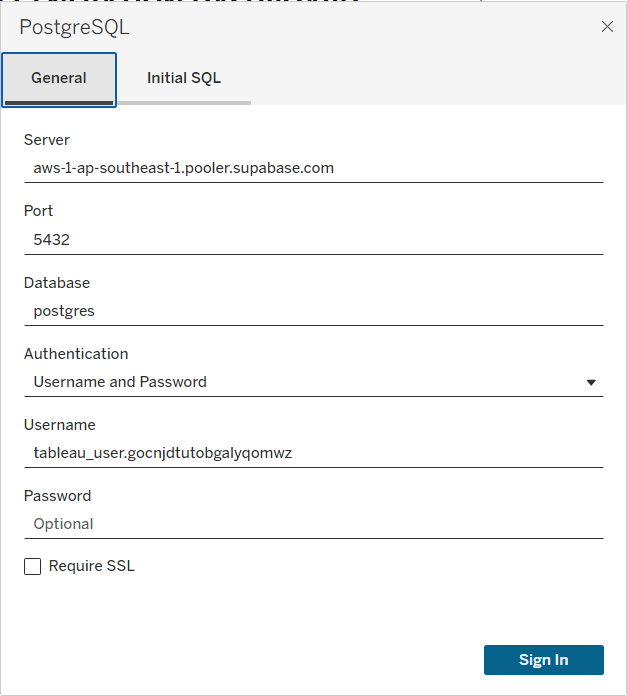
\includegraphics[width=0.62\textwidth]{figures/tableau_connect_supabase.png}
    \caption{Cửa sổ cấu hình kết nối PostgreSQL từ Tableau Desktop tới Supabase Data Warehouse}
    \label{fig:tableau_connect_supabase}
\end{figure}

Thông số cấu hình kết nối chi tiết giữa Tableau và hệ cơ sở dữ liệu PostgreSQL của dự án được chuẩn hóa như trong Bảng~\ref{tab:tableau_connection_params}:

\begin{table}[H]
\centering
\small
\renewcommand{\arraystretch}{1.25}
\begin{tabularx}{\textwidth}{@{} l l X @{}}
\toprule
\textbf{Tham số Kết nối} & \textbf{Giá trị Cấu hình} & \textbf{Ý nghĩa Kỹ thuật \& Bảo mật} \\
\midrule
\textbf{Connector Type} & PostgreSQL & Trình kết nối hiệu năng cao tối ưu hóa riêng cho PostgreSQL/Tableau. \\
\textbf{Server / Host} & \texttt{aws-1-ap-southeast-1.pooler.supabase.com} & Cổng Supabase Connection Pooler (AWS Singapore) giúp duy trì kết nối ổn định và tái sử dụng connection pool. \\
\textbf{Port} & \texttt{5432} & Cổng mạng tiêu chuẩn dành cho giao thức PostgreSQL Session Pool. \\
\textbf{Database} & \texttt{postgres} & Cơ sở dữ liệu đích chứa các schema \texttt{bi\_mart}, \texttt{gold}, \texttt{dim}. \\
\textbf{Authentication} & Username and Password & Xác thực danh tính người dùng bằng phương thức mã hóa định danh. \\
\textbf{Username} & \texttt{tableau\_user.gocnjdtutobgalyqomwz} & Tài khoản dịch vụ chuyên dụng (Dedicated Service Account) được phân quyền Read-only tối thiểu (Principle of Least Privilege) trên schema \texttt{bi\_mart}. \\
\textbf{Encryption} & Require SSL / TLS & Bắt buộc mã hóa toàn bộ luồng truyền tải dữ liệu giữa máy trạm BI và máy chủ Supabase. \\
\bottomrule
\end{tabularx}
\caption{Thông số thiết lập kết nối PostgreSQL từ Tableau tới Supabase Data Warehouse.}
\label{tab:tableau_connection_params}
\end{table}

Việc sử dụng cổng Pooler kết hợp tài khoản dịch vụ phân quyền độc lập mang lại 3 ưu điểm kỹ thuật vượt trội:
\begin{enumerate}[label=\arabic*., leftmargin=*]
    \item \textbf{Khả năng Chịu tải Cao (Concurrency Handling):} Cơ chế Connection Pooling tự động điều phối hàng trăm truy vấn phân tích song song từ các Dashboard mà không làm tràn bộ nhớ RAM của cụm máy chủ Supabase.
    \item \textbf{Bảo mật Dữ liệu Nghiêm ngặt (Least Privilege):} Tài khoản \texttt{tableau\_user} chỉ được cấp quyền \texttt{SELECT} trên tầng BI Mart và các bảng Dimension, ngăn chặn hoàn toàn rủi ro can thiệp thay đổi cấu trúc bảng hoặc ghi đè dữ liệu.
    \item \textbf{Độ trễ Truy vấn Cực thấp (Low Latency):} Cụm máy chủ đặt tại Datacenter Singapore (\texttt{ap-southeast-1}) đảm bảo thời gian phản hồi truy vấn dưới 1,5 giây cho mọi thao tác lọc tương tác từ Việt Nam.
\end{enumerate}

\subsection{Mô hình Kết nối Dữ liệu Tầng BI Mart và Tableau Relationships}
\label{subsec:bi_mart_model}

Để đảm bảo tốc độ phản hồi tính toán thời gian thực trên Tableau mà không gây quá tải cho hệ quản trị cơ sở dữ liệu Supabase PostgreSQL, dự án không thực hiện truy vấn trực tiếp trên các bảng sự kiện thô 2,7 triệu dòng. Thay vào đó, hệ thống Tableau kết nối trực tiếp với tầng BI Mart đã được tối ưu hóa sẵn thông qua hai Materialized Views lõi:
\begin{itemize}
    \item \texttt{bi\_mart.mv\_bi\_mart\_hourly\_measures}: Lưu trữ toàn bộ các đo lường chi tiết theo từng giờ của 42 trạm phát, bao gồm sản lượng thực tế (\texttt{e\_hourly}), sản lượng chuẩn STC (\texttt{e\_stc\_hourly}), sản lượng kỳ vọng hiệu chỉnh nhiệt (\texttt{e\_expected}), hệ số hiệu suất (\texttt{pr\_actual}, \texttt{pr\_adjusted}), suy hao do nhiệt (\texttt{loss\_temp}), nhiệt độ ô pin (\texttt{t\_cell}), cùng các cờ báo động ngoại lai GMM-IF (\texttt{gmm\_if\_outlier\_flag}).
    \item \texttt{bi\_mart.mv\_bi\_mart\_daily\_kpis}: Lưu trữ các chỉ số tổng hợp cấp ngày, tích hợp sẵn các chỉ số lũy kế theo tuần (\texttt{wtd\_energy}), tháng (\texttt{mtd\_energy}), năm (\texttt{ytd\_energy}), doanh thu ước tính (\texttt{daily\_revenue}), chi phí tổn thất do thiếu hụt công suất (\texttt{cost\_of\_underperformance}), và lượng phát thải khí nhà kính giảm thiểu (\texttt{daily\_co2\_avoided}).
\end{itemize}

Các Materialized Views này kết nối logic với hệ thống các bảng chiều (\texttt{dim\_solar\_site}, \texttt{dim\_geography}, \texttt{dim\_date}, \texttt{dim\_weather\_type}) thông qua mô hình liên kết Tableau Relationships (1-N). Mô hình này bảo toàn ngữ cảnh phân tích đa chiều mà không làm nhân bản dòng dữ liệu (Fan-out problem), tối ưu hóa tốc độ tải trang dưới 2 giây cho mọi thao tác tương tác lọc và khoan sâu (Drill-down).

\subsection{Bảng màu Ngữ nghĩa và Nguyên tắc Thiết kế UI/UX}
\label{subsec:color_palette}

Giao diện hệ thống Dashboard trên Tableau được thiết kế theo tư duy hiện đại, tối giản (Minimalist \& Clean Layout) nhằm tối đa hóa tỷ số dữ liệu trên mực in (Data-Ink Ratio) và tuân thủ các quy luật nhận thức thị giác Gestalt. Toàn bộ hệ màu được chuẩn hóa theo cấu hình giao diện \texttt{tableau\_theme.json} và ánh xạ trực tiếp từ tệp Workbook \texttt{main\_fixed\_01.twb}, đảm bảo độ tương phản cao ($\ge 4.5:1$) theo tiêu chuẩn WCAG 2.1 AA.

\subsubsection{Hệ thống Bảng màu Đồng bộ (Color Palette System)}

Nhằm phân biệt rõ ràng giữa các luồng thông tin vận hành và trạng thái kỹ thuật, hệ màu trong Dashboard được chia thành 3 phân nhóm chức năng: Bảng màu Chủ đạo (Primary), Bảng màu Cảnh báo Ngữ nghĩa (Semantic Alert), và Dải màu Tuần tự cho Heatmap (Sequential Palette).

\begin{table}[H]
\centering
\small
\renewcommand{\arraystretch}{1.3}
\begin{tabularx}{\textwidth}{@{} l l c X @{}}
\toprule
\textbf{Nhóm chức năng} & \textbf{Tên màu \& Mã Hex} & \textbf{Mẫu màu} & \textbf{Chỉ số \& Thành phần Ứng dụng trong Workbook} \\
\midrule
\multirow{3}{*}{\textbf{Bảng màu Chủ đạo}} 
& Classic Blue (\texttt{\#4E79A7}) & \textcolor{tblNavy}{\rule{1.2cm}{0.3cm}} & BANs sản lượng, đường xu hướng sản lượng thực tế ($e_{\text{hourly}}$), thanh Header. \\
& Solar Orange (\texttt{\#F28E2B}) & \textcolor{tblOrange}{\rule{1.2cm}{0.3cm}} & Bức xạ sóng ngắn (\texttt{shortwave\_radiation}), nhiệt độ môi trường, đường nhiệt ô pin. \\
& Eco Green (\texttt{\#59A14F}) & \textcolor{tblGreen}{\rule{1.2cm}{0.3cm}} & Hệ số công suất (Capacity Factor CF), thanh sản lượng lũy kế WTD/MTD/YTD. \\
\midrule
\multirow{4}{*}{\textbf{Cảnh báo Ngữ nghĩa}}
& Active/Success (\texttt{\#59A14F}) & \textcolor{tblGreen}{\rule{1.2cm}{0.3cm}} & Trạng thái tối ưu: $PR \ge 75\%$, tỷ lệ hoàn thành kế hoạch $\text{Yield Ratio} \ge 100\%$. \\
& Warning (\texttt{\#EDC948}) & \textcolor{tblYellow}{\rule{1.2cm}{0.3cm}} & Cảnh báo suy giảm nhẹ ($50\% \le PR < 75\%$), nhiệt độ ô pin vượt ngưỡng tối ưu $25^\circ\text{C}$. \\
& Danger/Outlier (\texttt{\#E15759}) & \textcolor{tblRed}{\rule{1.2cm}{0.3cm}} & \textbf{Độc quyền} đánh dấu cờ bất thường GMM-IF, vết rò rỉ điện ban đêm ($E > 0$), sụt giảm nặng. \\
& Adjusted/Ref (\texttt{\#76B7B2}) & \textcolor{tblTeal}{\rule{1.2cm}{0.3cm}} & Đường hiệu suất hiệu chỉnh nhiệt ($PR_{\text{adjusted}}$), sản lượng kỳ vọng ($E_{\text{expected}}$). \\
\midrule
\multirow{2}{*}{\textbf{Dải màu Phân tích}}
& Sequential Heatmap & \textcolor{tblSeqWarm}{\rule{1.2cm}{0.3cm}} & Dải màu \texttt{orange\_10\_0} chuyển từ Vàng nhạt (\texttt{\#F9E9E0}) sang Đỏ (\texttt{\#E15759}) trên Heatmap. \\
& Neutral Gray (\texttt{\#79706E}) & \textcolor{tblGray}{\rule{1.2cm}{0.3cm}} & Đường chuẩn tham chiếu (Reference Lines), trục tọa độ, nhãn thông số phụ trợ. \\
\bottomrule
\end{tabularx}
\caption{Quy chuẩn hệ thống màu sắc và ứng dụng thực tế trong Tableau Workbook \texttt{main\_fixed\_01.twb}.}
\label{tab:tableau_color_system}
\end{table}

\subsubsection{Nguyên tắc Bố cục Thị giác và Cấu trúc Khung Thẻ (Card-Based Container Layout)}

Bên cạnh hệ thống màu sắc, trải nghiệm tương tác trên Dashboard được tối ưu hóa thông qua các nguyên tắc thiết kế chuyên sâu:
\begin{itemize}[noitemsep]
    \item \textbf{Cấu trúc Phân tầng F-Pattern:} Mắt người dùng tự nhiên quét từ góc trên bên trái sang phải và xuống dưới. Do đó, các thẻ chỉ số cốt lõi (BANs) như \texttt{KPI total gen}, \texttt{AVG CF}, \texttt{KPI PR} được đặt tại dải trên cùng (Top Banner) với kích thước chữ lớn (18--24pt) để người quản lý nắm bắt nhanh tình trạng hệ thống chỉ trong vài giây đầu tiên.
    \item \textbf{Bố cục Khung Thẻ Phân Khu (Card-Based Container Layout):} Bố cục trực quan của dự án sử dụng các khung thẻ container riêng biệt có viền xám nhẹ thanh lịch (\texttt{\#E2E8F0}) trên nền sáng để nhóm các thành phần phân tích có liên quan về mặt logic (Khối thẻ KPI tổng hợp, Khối phân bố địa lý theo khuôn viên, Khối biểu đồ chuỗi thời gian sản lượng, Khối ma trận nhiệt tổn thất và Bảng xếp hạng thiết bị biến tần). Việc phân định bằng khung viền thẻ giúp người dùng dễ dàng định vị các vùng thông tin chức năng mà không bị rối mắt.
    \item \textbf{Tối ưu hóa Tỷ lệ Mực Thông tin (Data-Ink Ratio):} Bên trong mỗi thẻ biểu đồ, các đường lưới phụ (minor gridlines) được làm mờ hoặc loại bỏ, chỉ giữ lại các mốc tọa độ chính yếu và đường gốc (Zero-line) với tông màu xám rất nhạt (\texttt{\#E0E0E0}), giúp mắt người xem tập trung tối đa vào hình dáng biến thiên của đường cong sản lượng và các điểm dị thường nổi bật.
    \item \textbf{Đồng bộ Bộ lọc Toàn cục (Synchronized Global Filtering):} Toàn bộ bộ lọc theo Trạm (\texttt{Site Name}), Khoảng thời gian (\texttt{Date Range}), và Loại thời tiết (\texttt{Weather Type}) được bố trí gọn gàng tại bảng điều khiển bên phải (Right-panel) dưới dạng Dropdown, tự động đồng bộ hóa trên toàn bộ 3 Dashboard.
\end{itemize}

\subsection{Các Trường Tính toán Nghiệp vụ Bổ sung trên Tableau (Calculated Fields)}
\label{subsec:calculated_fields}

Để đáp ứng các yêu cầu phân tích kinh doanh đa chiều và các biểu đồ trực quan động trên Tableau, nhóm đã thiết lập một hệ sinh thái các Trường tính toán (Calculated Fields) chuyên sâu trong tệp tin \texttt{main\_fixed\_01.twb}. Bảng~\ref{tab:tableau_calculated_fields} tổng hợp các công thức tính toán nghiệp vụ cốt lõi:

\begin{table}[H]
\centering
\small
\renewcommand{\arraystretch}{1.25}
\begin{tabularx}{\textwidth}{@{} l p{5.5cm} X @{}}
\toprule
\textbf{Tên Trường Tính toán} & \textbf{Công thức Tableau} & \textbf{Ý nghĩa Nghiệp vụ} \\
\midrule
\texttt{[PR Actual]} & 
\texttt{SUM(IF [shortwave\_radiation] >= 100 AND [p\_stc] > 0 THEN [e\_hourly] END) / SUM(IF [shortwave\_radiation] >= 100 AND [p\_stc] > 0 THEN [capacity\_kw] * ([shortwave\_radiation] / 1000.0) END)} & 
Tính toán Hệ số Hiệu suất (PR) thực tế có điều kiện, loại bỏ các khoảng thời gian bức xạ yếu dưới $100\,\text{W/m}^2$ khi biến tần chưa kích hoạt phát điện. \\
\midrule
\texttt{[Weighted CF Trend]} & 
\texttt{SUM([e\_hourly]) / SUM([p\_stc])} & 
Hệ số công suất gia quyền theo tổng quy mô lắp đặt, phản ánh mức độ huy động công suất thực tế của toàn trạm. \\
\midrule
\texttt{[Number of Inverter]} & 
\texttt{IF CONTAINS(LOWER([inverter]), 'x') THEN INT(TRIM(SPLIT(LOWER([inverter]), 'x', 1))) ELSE 1 END} & 
Tách số lượng biến tần từ chuỗi văn bản kỹ thuật (ví dụ: \texttt{2x Fronius Symo 20.0}). \\
\midrule
\texttt{[kWh/inverter]} & 
\texttt{[e\_hourly] / [Number of Inverter]} & 
Sản lượng chuẩn hóa trên mỗi đầu biến tần, hỗ trợ so sánh hiệu quả giữa các dòng thiết bị khác nhau. \\
\midrule
\texttt{[kWh/panel]} & 
\texttt{[e\_hourly] / [number\_of\_panels]} & 
Sản lượng trung bình trên mỗi tấm pin, hỗ trợ nhận diện các chuỗi pin bị che bóng hoặc suy thoái. \\
\midrule
\texttt{[Outlier Hours SM/PM]} & 
\texttt{SUM(IF MONTH([full\_date]) = [Param Month] AND [gmm\_if\_outlier\_flag] = TRUE THEN 1 ELSE 0 END)} & 
Tính tổng số giờ xuất hiện dị thường trong tháng được chọn (SM) và tháng liền kề trước đó (PM). \\
\midrule
\texttt{[Outlier Hours MoM \%]} & 
\texttt{([Outlier Hours SM] - [Outlier Hours PM]) / ZN([Outlier Hours PM])} & 
Tốc độ tăng trưởng số giờ dị thường theo tháng (Month-over-Month), phản ánh mức độ gia tăng sự cố vận hành. \\
\midrule
\texttt{[Outlier MoM \% (Up/Down)]} & 
\texttt{IF [Outlier Hours MoM \%] > 0 THEN [Outlier Hours MoM \%] END} & 
Phân nhánh điều kiện để gán màu trực quan (màu đỏ khi sự cố tăng, màu xanh khi sự cố giảm) trên thẻ KPI. \\
\bottomrule
\end{tabularx}
\caption{Bảng tổng hợp các Trường tính toán nghiệp vụ (Calculated Fields) thiết lập trên Tableau.}
\label{tab:tableau_calculated_fields}
\end{table}

\section{Chi tiết Hệ thống Dashboard Phân tích}
\label{sec:dashboard_details}

Hệ thống trực quan hóa của dự án được đóng gói hoàn chỉnh trong tệp tin Tableau Workbook \texttt{reports/dashboards/main\_fixed\_01.twb}, bao gồm 3 Dashboard chuyên biệt được kết nối chặt chẽ theo luồng phân tích nguyên nhân - kết quả.

\subsection{Dashboard 1: Executive Overview (Tổng quan Vận hành \& Sức khỏe Hệ thống)}
\label{subsec:db_overview}

Dashboard \textit{Executive Overview} đóng vai trò là trung tâm chỉ huy dành cho Ban Giám đốc và các nhà quản lý dự án, cung cấp bức tranh toàn cảnh về sản lượng, doanh thu và sức khỏe vận hành của toàn bộ 42 trạm điện mặt trời tại Úc.

\begin{figure}[H]
    \centering
    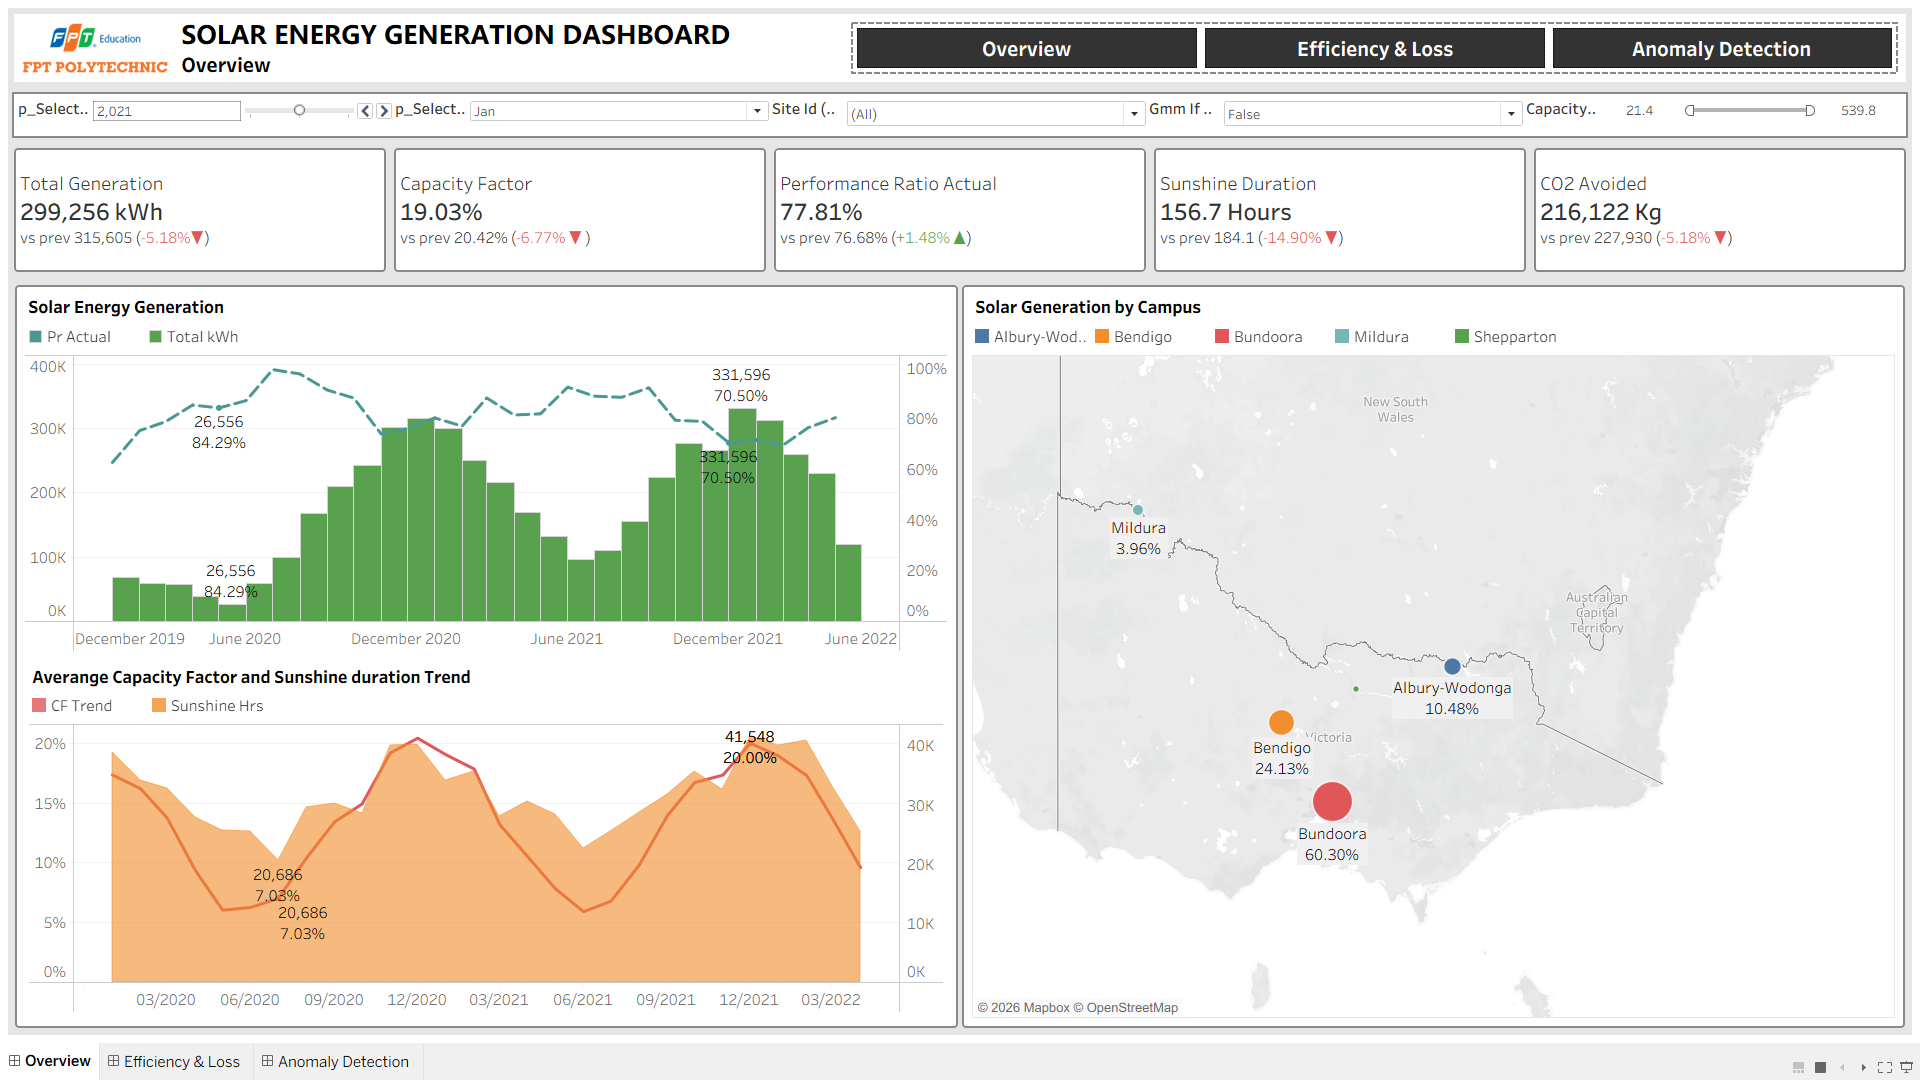
\includegraphics[width=0.95\textwidth]{figures/Dashboard_overview.png}
    \caption{Giao diện Dashboard 1: Executive Overview trên Tableau}
    \label{fig:dashboard_overview}
\end{figure}

Các thành phần giao diện và chỉ số phân tích chính bao gồm:
\begin{enumerate}[label=\alph*., leftmargin=*]
    \item \textbf{Thẻ Chỉ số Cốt lõi (BANs Layer):}
    \begin{itemize}
        \item \texttt{KPI total gen}: Hiển thị tổng sản lượng điện phát lũy kế ($E_{\text{actual}}$) tính bằng MWh/GWh, tích hợp so sánh tốc độ tăng trưởng MoM/YoY.
        \item \texttt{AVG CF}: Hệ số công suất khai thác trung bình ($\text{Capacity Factor} = \sum E / (P_{\text{stc}} \cdot 24)$).
        \item \texttt{KPI PR \& PR adjust}: Chỉ số hiệu suất thực tế ($PR_{\text{actual}}$) và chỉ số hiệu suất đã hiệu chỉnh nhiệt độ ($PR_{\text{adjusted}}$).
        \item \texttt{KPI Co2 avoided \& Sunshine dur}: Tổng khối lượng khí thải $\text{CO}_2$ triệt tiêu (kg), số cây xanh tương đương được trồng mới và tổng thời lượng nắng tích tụ trong kỳ.
    \end{itemize}

    \item \textbf{Bản đồ Địa lý Phân bố Trạm (Campus Map):}
    Trực quan hóa vị trí địa lý thực tế của 42 trạm PV tại các cơ sở đào tạo (Campus). Kích thước hình tròn (Symbol size) đại diện cho công suất thiết kế ($P_{\text{stc}}$ tính bằng $kWp$), trong khi màu sắc (Color gradient) phản ánh trực tiếp hệ số công suất CF. Nhờ đó, người quản lý lập tức nhận diện được các vùng địa lý có hiệu suất khai thác kém bất thường.

    \item \textbf{Ma trận Hiệu suất Trạm (Site Performance Matrix \& Consistency):}
    Biểu đồ xếp hạng phân bổ sản lượng ($gen/panel$) và độ ổn định vận hành giữa 42 trạm. Hệ thống trực quan hóa sự chênh lệch sản lượng trên từng tấm pin, giúp phát hiện các trạm đang hoạt động dưới mức tiềm năng thiết kế.

    \item \textbf{Xu hướng Sản lượng Tổng hợp (Total Generation \& Trend):}
    Biểu đồ đường/miền (Line/Area Chart) thể hiện sự biến đổi sản lượng theo thời gian (ngày, tháng) kết hợp phân tích đóng góp sản lượng theo từng chủng loại tấm pin (Panel Brands/Models).
\end{enumerate}

\subsection{Dashboard 2: Operational Efficiency \& Loss Analysis (Hiệu suất Vận hành \& Phân rã Tổn thất)}
\label{subsec:db_efficiency}

Dashboard \textit{Efficiency \& Loss} được thiết kế dành riêng cho đội ngũ kỹ sư kỹ thuật năng lượng nhằm ``giải thích'' nguyên nhân gốc rễ gây sụt giảm sản lượng, đặc biệt là hiện tượng suy hao do nhiệt độ (Thermal Degradation) và hiệu suất biến tần (Inverter/Optimizer).

\begin{figure}[H]
    \centering
    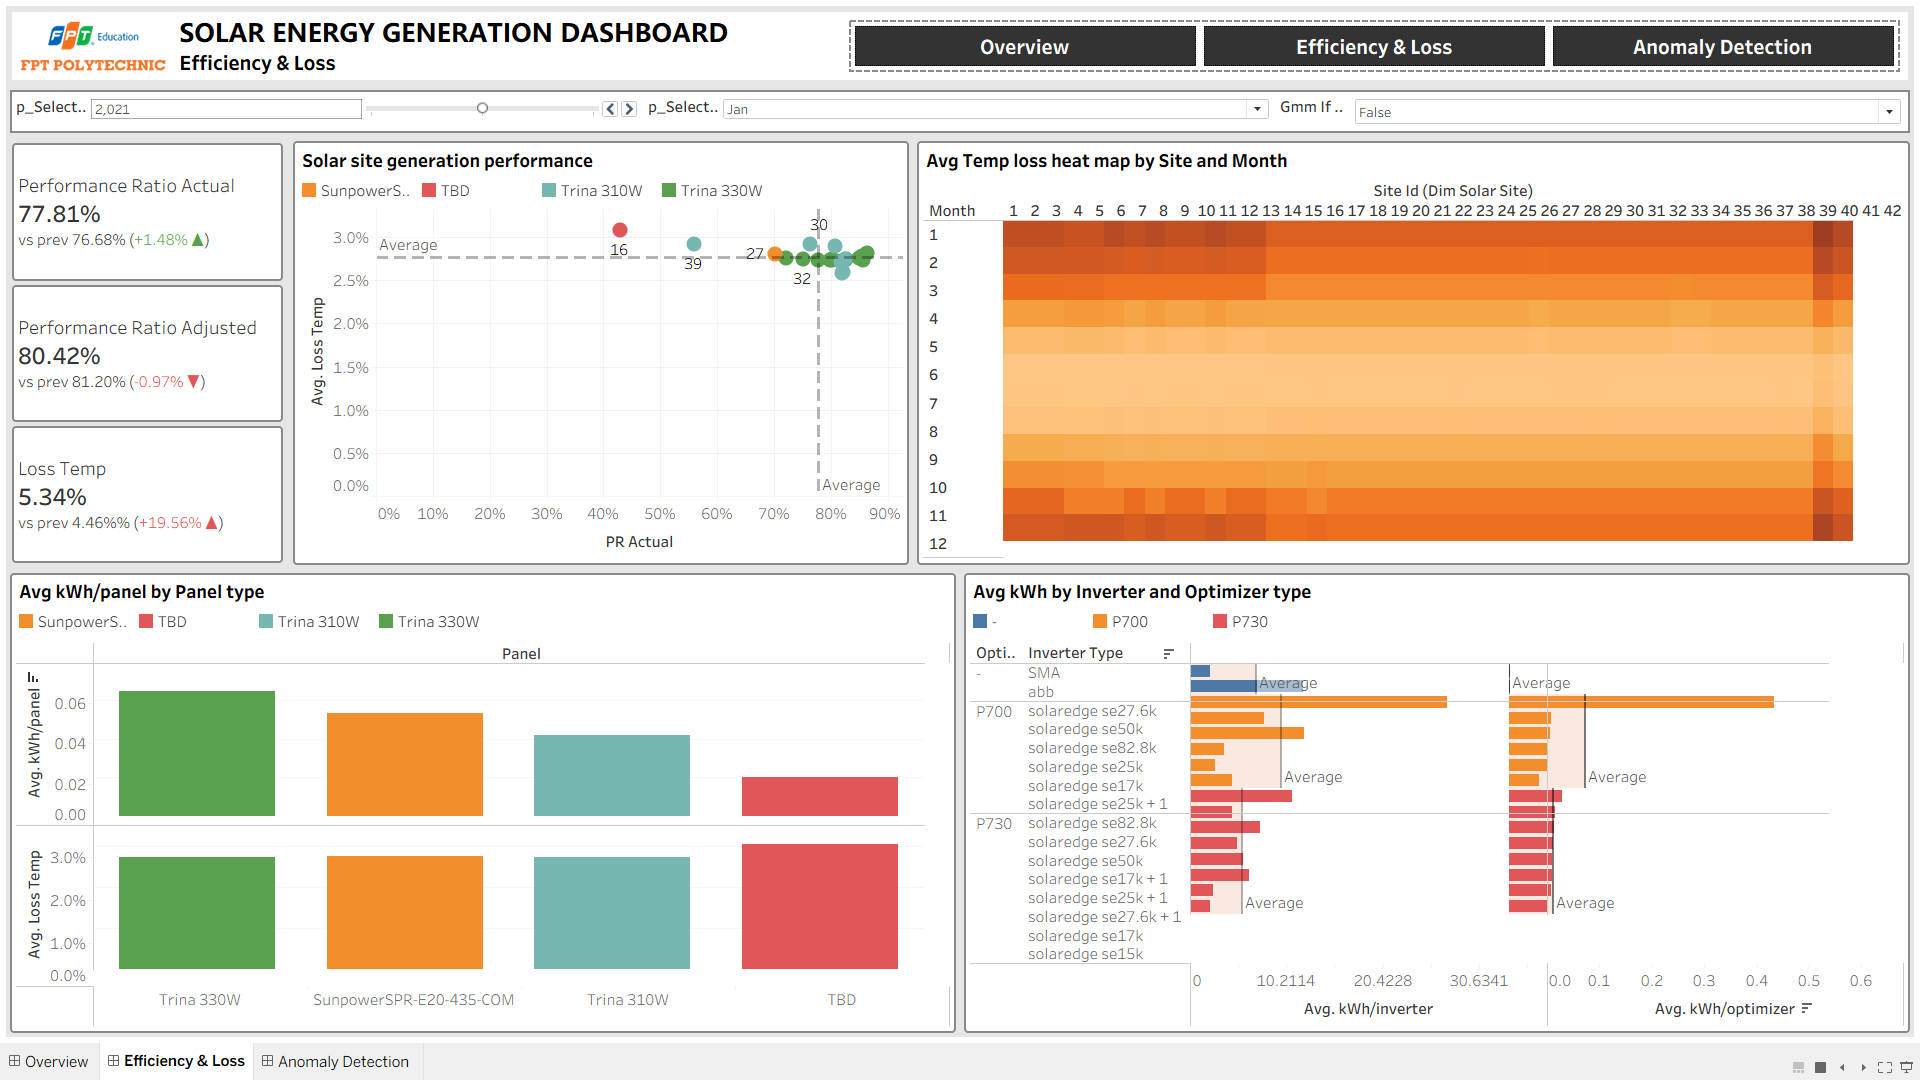
\includegraphics[width=0.95\textwidth]{figures/dashboard_efficiency_and_loss.png}
    \caption{Giao diện Dashboard 2: Operational Efficiency \& Loss Analysis trên Tableau}
    \label{fig:dashboard_efficiency}
\end{figure}

Các phân tích kỹ thuật chuyên sâu trên Dashboard bao gồm:
\begin{enumerate}[label=\alph*., leftmargin=*]
    \item \textbf{Đồ thị Xu hướng Tổn thất Nhiệt (Generation \& Loss Trend):}
    Sử dụng biểu đồ 2 trục tọa độ độc lập (Dual-Axis Chart) kết hợp giữa Sản lượng điện thực tế ($e_{\text{hourly}}$), Bức xạ sóng ngắn mặt trời (\texttt{shortwave\_radiation}) và Nhiệt độ ô pin ($T_{\text{cell}}$). Biểu đồ chứng minh luận điểm kỹ thuật quan trọng: Vào các khung giờ giữa trưa khi bức xạ đạt đỉnh cực đại ($> 800 \, \text{W/m}^2$), nhiệt độ ô pin tăng cao vượt quá $45^\circ\text{C}$ làm đường cong sản lượng bị chững lại hoặc suy giảm đáng kể so với mức lý thuyết.

    \item \textbf{Lưới Nhiệt Suy hao Nhiệt độ (Temperature Loss Heatmap \& Loss by Month):}
    Bản đồ nhiệt (Heatmap) thể hiện tỷ lệ tổn thất nhiệt độ trung bình (\texttt{avg\_loss\_temp}) phân rã theo 12 tháng trong năm và theo từng trạm phát. Dải màu chuyển từ Vàng nhạt (tổn thất $< 3\%$) sang Đỏ thẫm (tổn thất $> 8\%$), chỉ ra chính xác các tháng mùa hè đỉnh điểm cần tăng cường giải pháp làm mát hoặc thông gió bề mặt pin.

    \item \textbf{Đánh giá Hiệu suất Thiết bị (Inverter \& Optimizer Efficiency Rank):}
    Trực quan hóa chỉ số sản lượng trung bình trên mỗi tấm pin ($kWh/panel$) và tỷ lệ đáp ứng sản lượng kỳ vọng (\texttt{Yield ratio} $= E_{\text{actual}} / E_{\text{expected}}$) phân loại theo các hãng chế tạo Inverter và Optimizer. Phân tích này hỗ trợ đội ngũ bảo trì đánh giá chất lượng thiết bị vật lý thực tế để đưa ra quyết định thay thế hoặc bảo hành linh kiện.
\end{enumerate}

\subsection{Dashboard 3: Anomaly Detection \& Predictive Maintenance (Giám sát Bất thường \& Bảo trì Cảnh báo)}
\label{subsec:db_anomaly}

Dashboard \textit{Anomaly Detection} đóng vai trò là hệ thống cảnh báo sớm (Early Warning System) cho đội ngũ O\&M, trực quan hóa toàn bộ các cờ bất thường được phát hiện từ mô hình học máy GMM-IF và thuật toán Rolling IQR.

\begin{figure}[H]
    \centering
    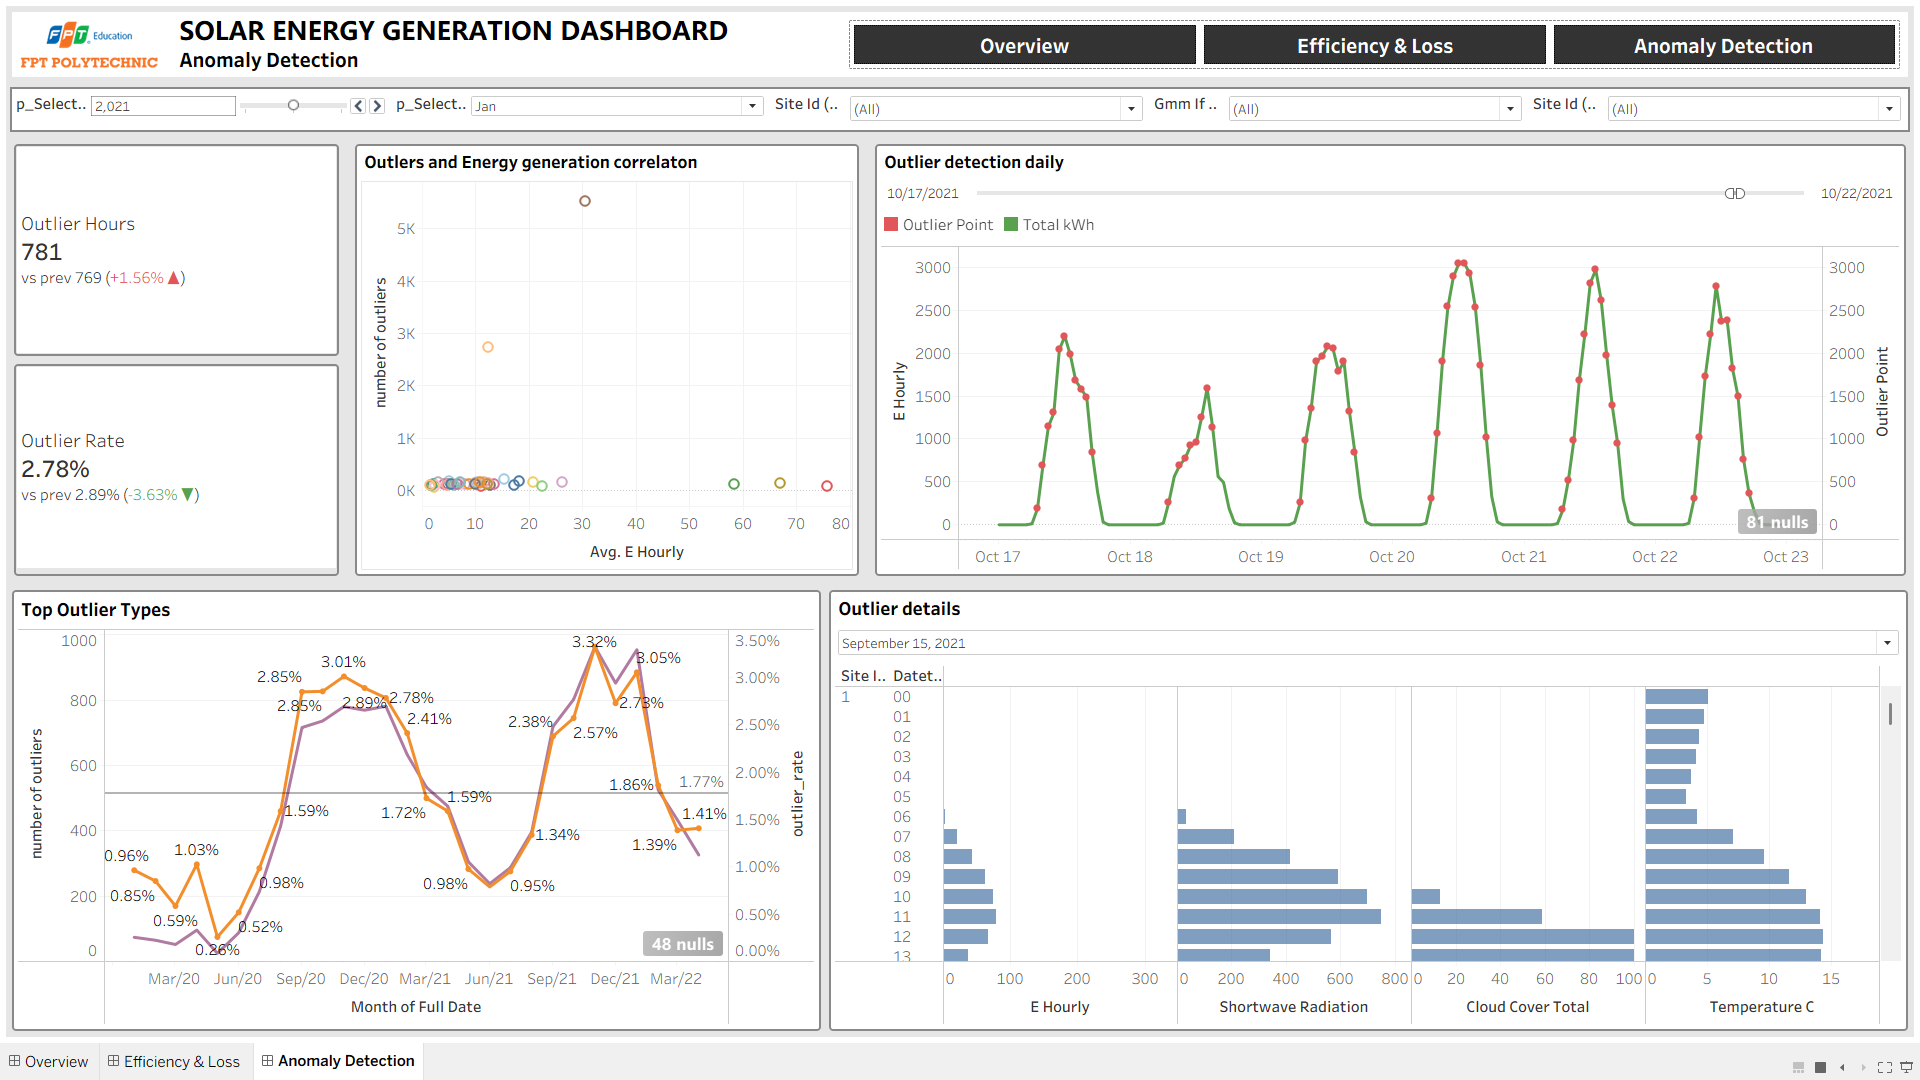
\includegraphics[width=0.95\textwidth]{figures/dashboard_anomaly_detection.png}
    \caption{Giao diện Dashboard 3: Anomaly Detection \& Predictive Maintenance trên Tableau}
    \label{fig:dashboard_anomaly}
\end{figure}

Các tính năng giám sát bất thường trọng tâm bao gồm:
\begin{enumerate}[label=\alph*., leftmargin=*]
    \item \textbf{Thẻ Thống kê Bất thường (Anomaly KPIs):}
    Hiển thị tổng số giờ phát hiện bất thường (\texttt{KPI Outlier Hours}), tỷ lệ phần trăm dữ liệu dị thường (\texttt{KPI Outlier Rate}), số lượng bản ghi gắn cờ (\texttt{number of outliers}) và chỉ số biến động so với tháng trước (\texttt{Outlier Rate MoM \%}).

    \item \textbf{Biểu đồ Chuỗi thời gian Phát hiện Dị thường (Time-series Outlier Detect):}
    Đồ thị chuỗi thời gian liên tục 15 phút biểu diễn sản lượng điện. Tất cả các mốc thời gian bị mô hình GMM-IF gắn cờ bất thường (\texttt{gmm\_if\_outlier\_flag = true}) được đánh dấu bằng các điểm nút tròn màu Đỏ rực (\texttt{\#E15759}) trên nền đường line sản lượng. Kỹ sư có thể nhấp chuột trực tiếp vào điểm dị thường để mở thẻ thông tin chi tiết (Tooltip) hiển thị lý do bất thường (\texttt{gmm\_if\_outlier\_reason}).

    \item \textbf{Bản đồ Nhiệt Phát hiện Rò rỉ Điện Ban đêm (Outlier by Site Heatmap):}
    Bản đồ nhiệt 2 chiều với Trục tung đại diện cho 24 khung giờ trong ngày ($0 - 23h$) và Trục hoành đại diện cho 42 trạm phát. 
    
    Quy tắc trực quan hóa áp đặt điều kiện đặc biệt: Nếu trong khung giờ ban đêm từ 18:30 đến 05:30 xuất hiện giá trị sản lượng $E > 0$, ô tương ứng sẽ lập tức bị tô màu Đỏ đậm. Đây là bằng chứng trực quan trực tiếp phát hiện sự cố rò rỉ dòng điện ngược (Reverse Current) hoặc cảm biến đo đạc CT bị sai lệch mốc 0 (Zero-drift fault), giúp kỹ sư khoanh vùng vị trí sự cố ngay lập tức.

    \item \textbf{Chi tiết Cảnh báo Phân loại Lỗi (Outlier Type \& Details):}
    Bảng thống kê chi tiết danh sách trạm và phân loại nhóm nguyên nhân dị thường (\textit{Dòng rò ban đêm}, \textit{Extreme Power Spike}, \textit{Sensor Freeze}, \textit{Daytime Sudden Drop}), hỗ trợ lập danh mục ưu tiên cho các đội kỹ thuật đi kiểm tra hiện trường.
\end{enumerate}

\begin{thebibliography}{99}
\addcontentsline{toc}{chapter}{Tài liệu Tham khảo}

% --- I. Nguồn Dữ liệu Dự án và Công trình Nghiên cứu Gốc ---
\bibitem{wimalaratne2022unisolar}
S.~Wimalaratne, D.~Haputhanthri, S.~Kahawala, G.~Gamage, D.~Alahakoon, và A.~Jennings,
\newblock ``UNISOLAR: An Open Dataset of Photovoltaic Solar Energy Generation in a Large Multi-Campus University Setting,''
\newblock \textit{15th International Conference on Human System Interaction (HSI)}, IEEE, 2022.
\newblock DOI: \href{https://doi.org/10.1109/HSI55341.2022.9869474}{10.1109/HSI55341.2022.9869474}.

\bibitem{openmeteo2023}
Open-Meteo,
\newblock ``Historical Weather API \& ERA5/ERA5-Land Reanalysis Climate Dataset,''
\newblock \textit{Open-Meteo Documentation}, 2023. [Online]. Available: \url{https://open-meteo.com/}.

\bibitem{iea2023pvps}
IEA-PVPS Task 13,
\newblock ``Performance, Operation and Reliability of Photovoltaic Systems: Review of Failures and Degradation Mechanisms,''
\newblock \textit{International Energy Agency Technical Report}, IEA-PVPS T13-15:2023, 2023.

% --- II. Thuật toán Phát hiện Bất thường và Xử lý Dữ liệu ---
\bibitem{li2025gmmif}
X.~Li, G.~Du, Y.~Li, Z.~Ma, L.~Liu, M.~Jiang, F.~Liu, và T.~Mu,
\newblock ``Outlier Detection of Photovoltaic Power Generation System Data Based on GMM-IF Algorithm,''
\newblock \textit{IEEE Access}, vol.~13, pp.~108823--108837, 2025.
\newblock DOI: \href{https://doi.org/10.1109/ACCESS.2025.3581641}{10.1109/ACCESS.2025.3581641}.

\bibitem{liu2008isolation}
F.~T.~Liu, K.~M.~Ting, và Z.-H.~Zhou,
\newblock ``Isolation Forest,''
\newblock trong \textit{Proceedings of the IEEE International Conference on Data Mining (ICDM)}, 2008, pp.~413--422.

\bibitem{bishop2006pattern}
C.~M.~Bishop,
\newblock \textit{Pattern Recognition and Machine Learning},
\newblock Springer, New York, 2006.

\bibitem{tukey1977eda}
J.~W.~Tukey,
\newblock \textit{Exploratory Data Analysis},
\newblock Addison-Wesley, Reading, MA, 1977.

\bibitem{chandola2009anomaly}
V.~Chandola, A.~Banerjee, và V.~Kumar,
\newblock ``Anomaly Detection: A Survey,''
\newblock \textit{ACM Computing Surveys}, vol.~41, no.~3, pp.~1--58, 2009.

\bibitem{kim2019missing}
T.~Kim, W.~Ko, và J.~Kim,
\newblock ``Analysis and Impact Evaluation of Missing Data Imputation in Day-ahead PV Generation Forecasting,''
\newblock \textit{Applied Sciences}, vol.~9, no.~1, p.~204, 2019.
\newblock DOI: \href{https://doi.org/10.3390/app9010204}{10.3390/app9010204}.

% --- III. Mô hình Dự báo Chuỗi Thời gian và Học máy ---
\bibitem{roy2025hourly}
M.~Roy, V.~Pyltsov, và Y.~Hu,
\newblock ``IISE PG\&E Energy Analytics Challenge 2025: Hourly-Binned Regression Models Beat Transformers in Load Forecasting,''
\newblock Columbia University, arXiv:2505.11390, 2025. [Online]. Available: \url{https://arxiv.org/abs/2505.11390}.

\bibitem{haurwitz1945}
B.~Haurwitz,
\newblock ``Insolation in Relation to Cloudiness and Cloud Density,''
\newblock \textit{Journal of Meteorology}, vol.~2, no.~3, pp.~154--166, 1945.

\bibitem{bailey2024}
M.~D.~Bailey và cộng sự,
\newblock ``Temporal and Spatial Downscaling for Solar Radiation,''
\newblock arXiv:2405.11046, 2024. [Online]. Available: \url{https://arxiv.org/abs/2405.11046}.

\bibitem{engerer2014kpv}
N.~A.~Engerer và F.~P.~Mills,
\newblock ``KPV: A clear-sky index for photovoltaics,''
\newblock \textit{Solar Energy}, vol.~105, pp.~679--693, 2014.
\newblock DOI: \href{https://doi.org/10.1016/j.solener.2014.04.019}{10.1016/j.solener.2014.04.019}.

\bibitem{dev2018tes}
S.~Dev, T.~AlSkaif, M.~Hossari, R.~Godina, A.~Louwen, và W.~van Sark,
\newblock ``Solar Irradiance Forecasting Using Triple Exponential Smoothing,''
\newblock trong \textit{IEEE International Conference on Smart Energy Systems and Technologies (SEST)}, 2018.
\newblock arXiv:1807.05872.

\bibitem{pin2025wape}
A.~Temporal-Neto và cộng sự,
\newblock ``PIN: A new metric to evaluate solar irradiance forecast models,''
\newblock \textit{Energy Reports}, vol.~13, pp.~1--12, 2025.
\newblock DOI: \href{https://doi.org/10.1016/j.egyr.2025.01.076}{10.1016/j.egyr.2025.01.076}.

\bibitem{lundberg2017shap}
S.~M.~Lundberg và S.-I.~Lee,
\newblock ``A Unified Approach to Interpreting Model Predictions,''
\newblock trong \textit{Advances in Neural Information Processing Systems (NeurIPS)}, vol.~30, 2017.
\newblock arXiv:1705.07874.

\bibitem{zhang2015metrics}
J.~Zhang, A.~Florita, B.-M.~Hodge, S.~Lu, H.~F.~Hamann, V.~Banunarayanan, và A.~M.~Brockway,
\newblock ``A suite of metrics for assessing the performance of solar power forecasting,''
\newblock \textit{Solar Energy}, vol.~111, pp.~157--175, 2015.
\newblock DOI: \href{https://doi.org/10.1016/j.solener.2014.10.016}{10.1016/j.solener.2014.10.016}.

\bibitem{zhang2013metrics}
J.~Zhang, B.-M.~Hodge, và A.~Florita,
\newblock ``Comprehensive Evaluation of Solar Irradiance and Power Forecasting Metrics,''
\newblock NREL/CP-5500-60142, \textit{3rd International Workshop on Integration of Solar Power into Power Systems}, 2013.

\bibitem{lonij2012tucson}
V.~P.~Lonij, A.~E.~Brooks, K.~Koch, và A.~D.~Cronin,
\newblock ``Analysis of 80 Rooftop PV Systems in the Tucson, AZ Area,''
\newblock trong \textit{38th IEEE Photovoltaic Specialists Conference (PVSC)}, 2012, pp.~549--553.
\newblock DOI: \href{https://doi.org/10.1109/PVSC.2012.6317674}{10.1109/PVSC.2012.6317674}.

\bibitem{taylor2018prophet}
S.~J.~Taylor và B.~Letham,
\newblock ``Forecasting at Scale,''
\newblock \textit{The American Statistician}, vol.~72, no.~1, pp.~37--45, 2018.

\bibitem{box2015time}
G.~E.~P.~Box, G.~M.~Jenkins, G.~C.~Reinsel, và G.~M.~Ljung,
\newblock \textit{Time Series Analysis: Forecasting and Control}, 5th ed.,
\newblock John Wiley \& Sons, Hoboken, NJ, 2015.

\bibitem{ke2017lightgbm}
G.~Ke, Q.~Meng, T.~Finley, T.~Wang, W.~Chen, W.~Ma, Q.~Ye, và T.-Y.~Liu,
\newblock ``LightGBM: A Highly Efficient Gradient Boosting Decision Tree,''
\newblock trong \textit{Advances in Neural Information Processing Systems (NeurIPS)}, vol.~30, 2017, pp.~3146--3154.

\bibitem{chen2016xgboost}
T.~Chen và C.~Guestrin,
\newblock ``XGBoost: A Scalable Tree Boosting System,''
\newblock trong \textit{Proceedings of the ACM SIGKDD International Conference on Knowledge Discovery and Data Mining}, 2016, pp.~785--794.

\bibitem{aivietnam2025dvc}
Đặng Nhã và Anh Dương,
\newblock ``Data Version Control,''
\newblock tài liệu bài giảng \textit{AI VIET NAM --- All-in-One 2025}, slide~9 (\textit{Theory Perspective --- ML Life Cycle}), 2025.

\bibitem{kolassa2007mad}
S.~Kolassa và W.~Schütz,
\newblock ``Advantages of the MAD/Mean ratio over the MAPE,''
\newblock \textit{Foresight: The International Journal of Applied Forecasting}, no.~6, pp.~40--43, 2007.

\bibitem{nguyen2026meta}
T.~N.~Nguyen và F.~Müsgens,
\newblock ``A meta-analysis of solar forecasting based on skill score,''
\newblock \textit{Journal of Renewable and Sustainable Energy}, vol.~18, no.~2, p.~026102, 2026.
\newblock DOI: \href{https://doi.org/10.1063/5.0300682}{10.1063/5.0300682}.

\bibitem{marquez2013skill}
R.~Marquez và C.~F.~M.~Coimbra,
\newblock ``Proposed Metric for Evaluation of Solar Forecasting Models,''
\newblock \textit{Journal of Solar Energy Engineering} (ASME), vol.~135, no.~1, p.~011016, 2013.
\newblock DOI: \href{https://doi.org/10.1115/1.4007496}{10.1115/1.4007496}.

\bibitem{wwrp2009verif}
WWRP/WGNE Joint Working Group on Forecast Verification Research,
\newblock ``Forecast Verification: Issues, Methods and FAQ,''
\newblock Bureau of Meteorology, Australia, 2009. [Online]. Available: \url{https://www.cawcr.gov.au/projects/verification/verif_web_page.html}.

% --- IV. Kiến trúc Kho Dữ liệu, API và Công cụ Trực quan hóa ---
\bibitem{kimball2013dwh}
R.~Kimball và M.~Ross,
\newblock \textit{The Data Warehouse Toolkit: The Definitive Guide to Dimensional Modeling}, 3rd ed.,
\newblock John Wiley \& Sons, Indianapolis, IN, 2013.

\bibitem{wmo2021guide}
World Meteorological Organization (WMO),
\newblock \textit{Guide to Instruments and Methods of Observation: Volume I -- Measurement of Meteorological Variables},
\newblock WMO-No. 8, Geneva, Switzerland, 2021.

\bibitem{supabase2024}
Supabase Inc.,
\newblock ``PostgreSQL Database \& Row-Level Security for Modern Analytics Architecture,''
\newblock \textit{Supabase Technical Architecture Documentation}, 2024. [Online]. Available: \url{https://supabase.com/docs}.

\bibitem{pedregosa2011sklearn}
F.~Pedregosa et~al.,
\newblock ``Scikit-learn: Machine Learning in Python,''
\newblock \textit{Journal of Machine Learning Research}, vol.~12, pp.~2825--2830, 2011.

\bibitem{tableau2023guidelines}
Tableau Software (Salesforce),
\newblock \textit{Visual Analysis Best Practices: A Guide to Creating Meaningful Dashboards},
\newblock Seattle, WA, 2023.

\end{thebibliography}


\end{document}
